\section{Results}

\Cref{fig:dem_ts_aug_04_2011}, \cref{fig:dem_ts_aug_31_2012} and \cref{fig:dem_ts_oct_28_2021} shows the timeseries plot of DEM for the three events. The time series plot is calculated by averaging the acceptable DEM solutions obtained for each image over three consecutive temperature range (i.e averaging the solutions for 5.85, 5.9 and 5.95 etc.). Blue curve corresponds to the full disk DEM and red curve corresponds to the point source DEM. The temperature range above logT=6.45 has been omitted as no correlation was found between point source and full disk.

% \begin{figure}[h!]
%     \centering
%     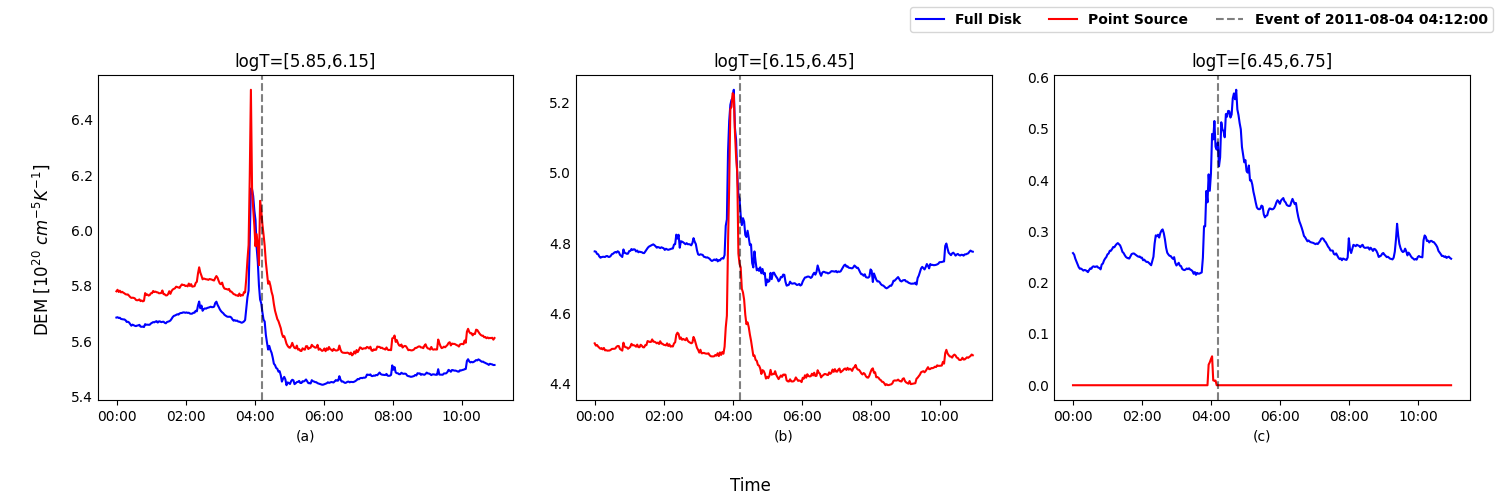
\includegraphics[width=\textwidth]{images/dem_ts_aug_04_2011.png}
%     \caption[DEM Timeseries for August 2011 Event]{Timeseries of DEM for \nth{4} August 2011 Event.}
%     \label{fig:dem_ts_aug_04_2011}
% \end{figure}

% \begin{figure}[h!]
%     \centering
%     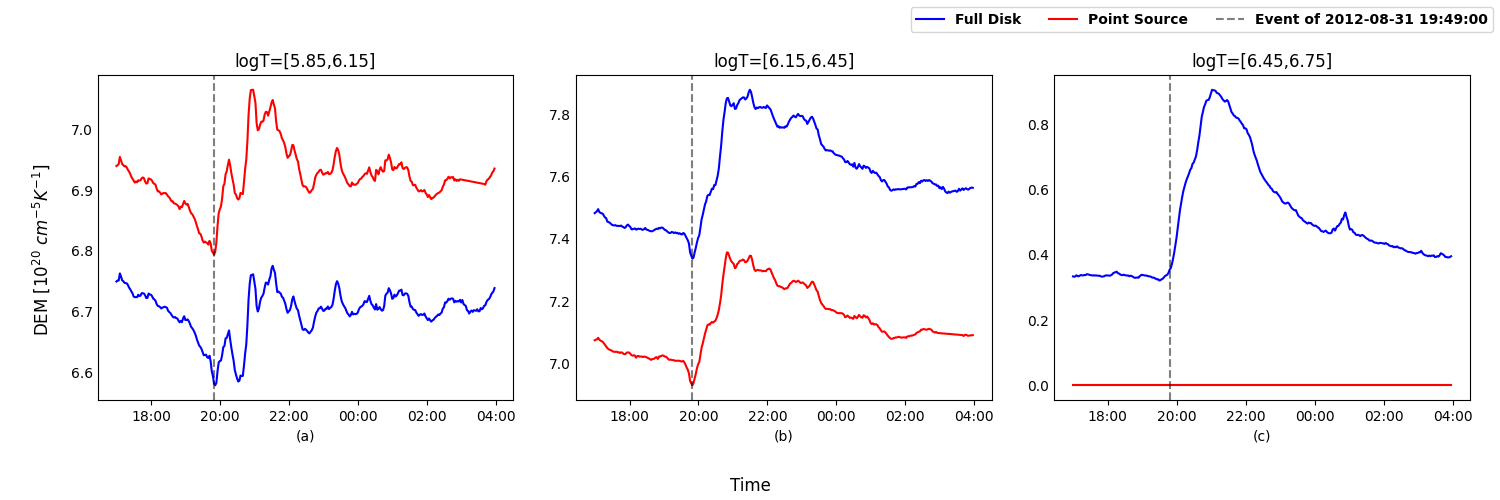
\includegraphics[width=\textwidth]{images/dem_ts_aug_31_2012.png}
%     \caption[DEM Timeseries for August 2012 Event]{Timeseries of DEM for \nth{4} August 2012 Event}
%     \label{fig:dem_ts_aug_31_2012}
% \end{figure}

\begin{figure}[h!]
    \centering
    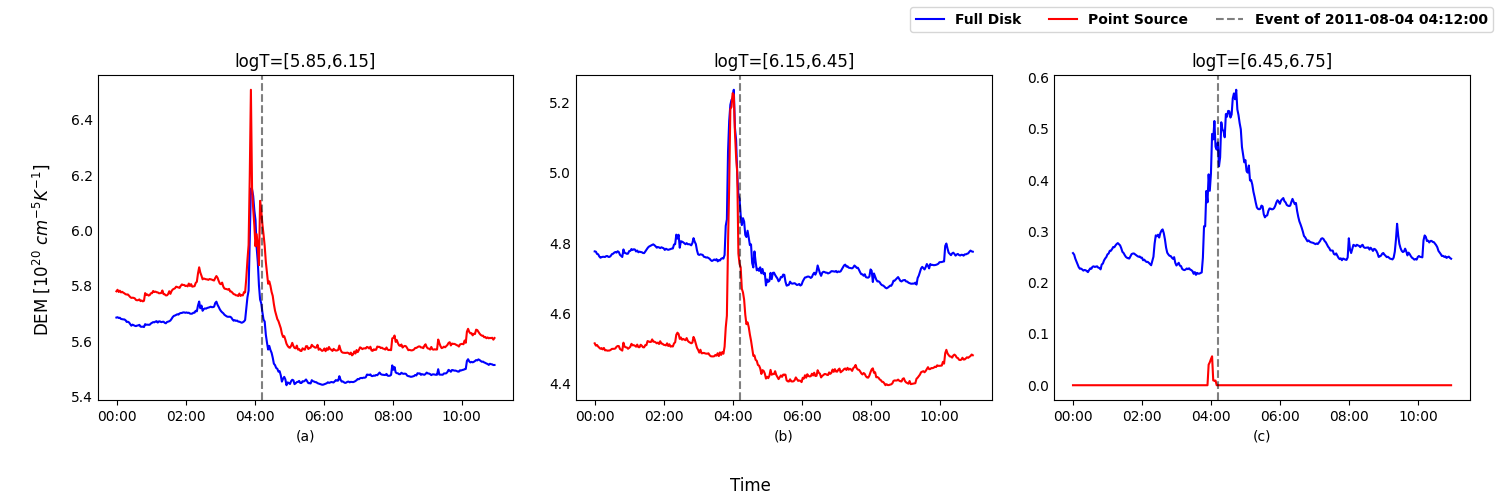
\includegraphics[width=\textwidth]{images/dem_ts_aug_04_2011.png}
    \caption[DEM Timeseries for August 2011 Event]{Timeseries of DEM for \nth{4} August 2011 Event.}
    \label{fig:dem_ts_aug_04_2011}
\end{figure}

\begin{figure}[h!]
    \centering
    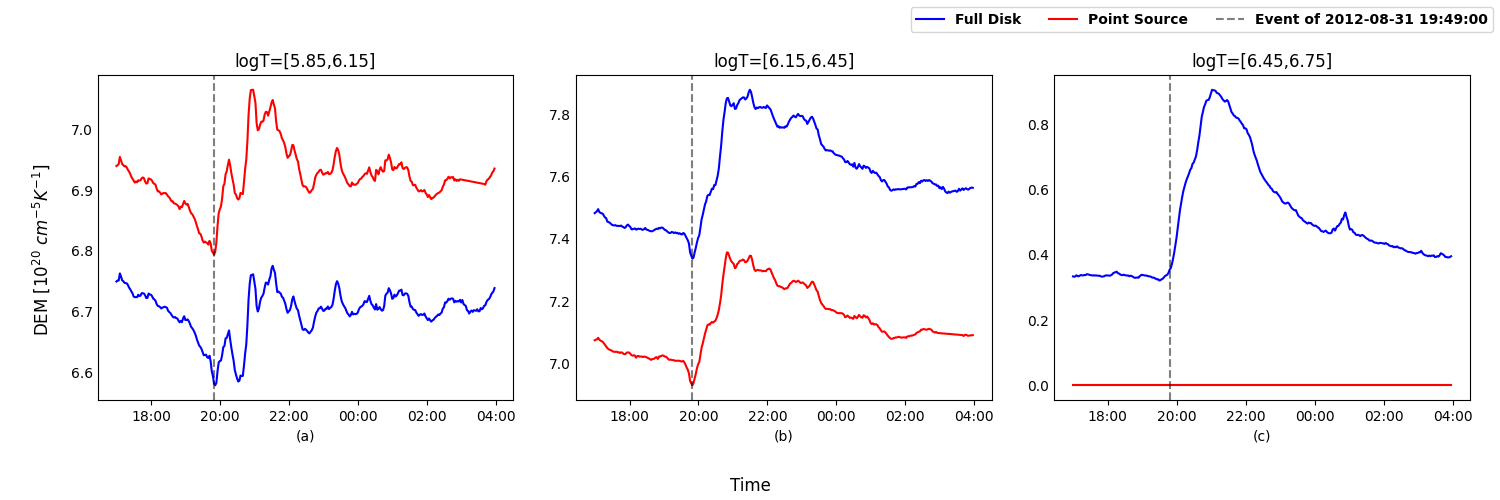
\includegraphics[width=\textwidth]{images/dem_ts_aug_31_2012.png}
    \caption[DEM Timeseries for August 2012 Event]{Timeseries of DEM for \nth{31} August 2012 Event}
    \label{fig:dem_ts_aug_31_2012}
\end{figure}

\begin{figure}[h!]
    \centering
    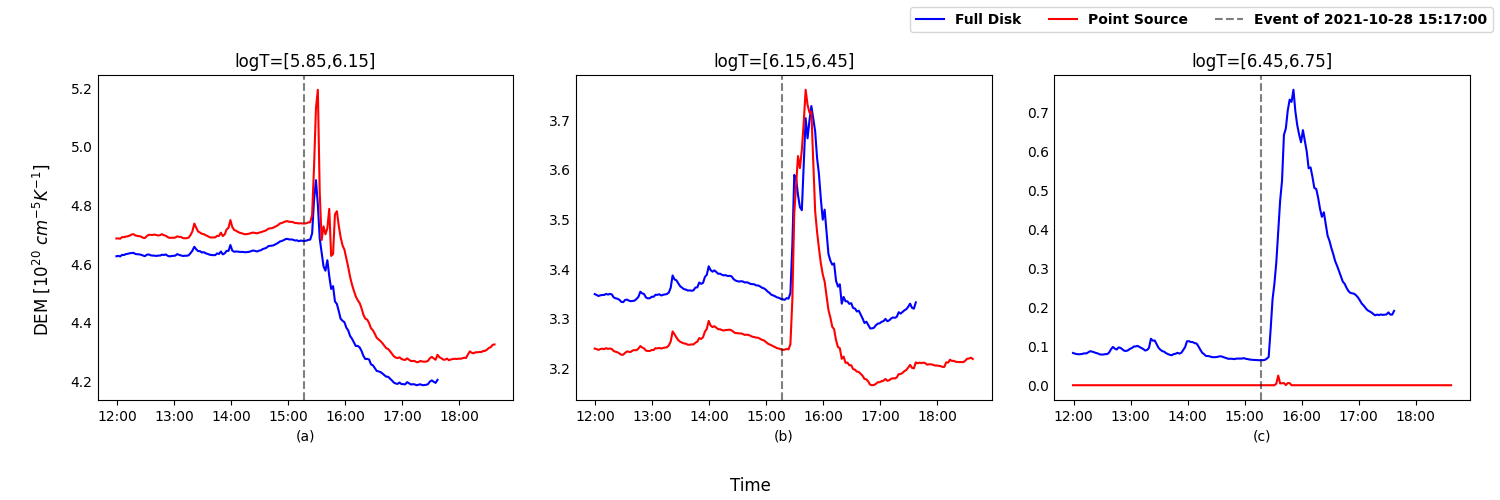
\includegraphics[width=\textwidth]{images/dem_ts_oct_28_2021.png}
    \caption[DEM Timeseries for October 2021 Event]{Timeseries of DEM for \nth{28} October 2021 Event}
    \label{fig:dem_ts_oct_28_2021}
\end{figure}

The sudden increase in the DEM curve is due to the solar flare which is associated with the CME. From the above figures, we can see that there is very high correlation for the first two temperature ranges, but there is little to no correlation in the DEM profiles of the full disk and point source for the temperature range logT=[6.45, 6.75]. For temperature ranges greater than logT=6.45, the correlation is almost 0. We make use of Pearson's Correlation coeffecient to find out the amount of correlation between the point source and full disk DEM, for which we use \texttt{pearsonr} function from the \texttt{scipy} library in Python.\\

\begin{table}
    \centering
    \begin{tblr}{
          cell{1}{1} = {r=2}{},
          cell{1}{2} = {c=3}{c},
          vline{1-5} = {-}{},
          hline{1-6} = {-}{},
        }
        Event        & Pearson Correlation Coeffecient &         & \\
        & logT=[5.85, 6.15]  & logT=[6.15, 6.45] & logT=[6.45, 6.75] \\
        August 2011  & 0.9449 & 0.9767 & 0.2190\\
        August 2012  &\\
        October 2021 & 0.9555 & 0.9577 & 0.2578 \\
    \end{tblr}
    \caption{Correlation between Point source and Full Disk DEM}
\end{table}

We see a discrepancy in the value of DEM between the point source and full disk average values. This could be due to the error induced during the DEM profile reconstruction, instrumental errors, error incurred during the resampling or reduction of image dimension from 4096 $\times$ 4096 pixels to 512 $\times$ 512 and it could also be due to averaging error. The dataset length is not equal in some of the case as invalid or small DEM solution values have been removed.

%%% Local Variables:
%%% mode: LaTeX
%%% TeX-master: "main"
%%% End:
